\documentclass{article}


\usepackage{amsmath,amssymb,amsthm,amsfonts,amscd}
\usepackage{multirow}
\usepackage{animate}
\usepackage{bbm}
\usepackage{enumerate}
\usepackage[tmargin=1in, bmargin=1in, lmargin=0.75in, rmargin=0.75in]{geometry}
\usepackage[colorlinks]{hyperref}
\usepackage{mathtools}
\usepackage[framemethod=tikz]{mdframed}
\usepackage{doi}
\usepackage{framed}
\usepackage{xcolor}
\usepackage{graphicx}
\usepackage{mathrsfs}
\usepackage{esvect}
\usepackage{commath}
\usepackage{lastpage}
\usepackage{mathpazo}
% \usepackage{tgpagella}
\usepackage{anyfontsize}
\usepackage{tkz-graph}
\usepackage[linesnumbered,ruled,vlined]{algorithm2e}
\usepackage[capitalize, nameinlink]{cleveref}
\newcommand\mycommfont[1]{\footnotesize\ttfamily{#1}}
\SetCommentSty{mycommfont}
\SetArgSty{textup}
\usepackage[square,numbers]{natbib}
\usepackage{verbatim}
\usepackage{titlesec}
\titleformat{\section}[block]{\sffamily\Large\filcenter\bfseries}{\S\thesection.}{0.25cm}{\Large}
\titleformat{\subsection}[block]{\large\bfseries\sffamily}{\thesubsection.}{0.2cm}{\large}
\titleformat{\subsubsection}[block]{\large\bfseries\sffamily}{\normalsize\thesubsubsection.}{0.15cm}{\normalsize}
\usepackage{listings} % For code listings

\colorlet{shadecolor}{black}
\lstnewenvironment{code}{%
\footnotesize
    \shaded
    \lstset{
        basicstyle=\ttfamily\color{white},
        backgroundcolor=\color{shadecolor},
        frame=single, % Add a frame around the code
        framerule=0pt, % No rule width for the frame
        framesep=4pt, % Adjust the spacing between frame and content
    }%
}{%
    \endshaded
}

\usepackage{fancyhdr}
% \renewcommand\thesubsection{\thesection.\alph{subsection}}

\Crefname{algocf}{Algorithm}{Algorithms}


\newcommand{\hr}[1]{\rule{\linewidth}{#1}}



\title{COL334 Assignment1}
\author{Ankit Mondal and Anish Banerjee}
\begin{document}
\maketitle

\section{Network Analysis}
\begin{enumerate}[a.]
    \item We ran {\tt tracert} on {\tt iitd.ac.in} outside IITD network and got the following output:
    \begin{code}
PS C:\Users\Anish> tracert iitd.ac.in

Tracing route to iitd.ac.in [103.27.9.24]
over a maximum of 30 hops:

 1    4 ms    3 ms    9 ms dsldevice.lan [192.168.1.1]
 2   87 ms   73 ms   26 ms abts-north-dynamic-255.187.69.182.airtelbroadband.in [182.69.187.255]
 3   34 ms   28 ms   48 ms 125.18.240.153
 4   38 ms   45 ms   38 ms 116.119.106.136
 5   47 ms   53 ms   49 ms 49.44.220.188
 6    *       *       *    Request timed out.
 7    *       *       *    Request timed out.
 8   47 ms   43 ms   47 ms 136.232.148.178
 9    *       *       *    Request timed out.
10    *       *       *    Request timed out.
11    *       *       *    Request timed out.
12   45 ms   59 ms   52 ms 103.27.9.24
13  187 ms   46 ms   61 ms 103.27.9.24
14   47 ms   48 ms   49 ms 103.27.9.24

Trace complete.
    \end{code}
    \item TODO
    \item We observe that the maximum packet size that can be sent is 68 (to {\tt google.com})
\begin{code}
root@IdeapadAB:/mnt/c/Users/Anish# ping -s 68 -c 5 google.com
PING google.com (142.250.194.238) 68(96) bytes of data.
76 bytes from del12s08-in-f14.1e100.net (142.250.194.238): icmp_seq=1 ttl=116 time=7.00 ms
76 bytes from del12s08-in-f14.1e100.net (142.250.194.238): icmp_seq=2 ttl=116 time=6.73 ms
76 bytes from del12s08-in-f14.1e100.net (142.250.194.238): icmp_seq=3 ttl=116 time=7.11 ms
76 bytes from del12s08-in-f14.1e100.net (142.250.194.238): icmp_seq=4 ttl=116 time=6.05 ms
76 bytes from del12s08-in-f14.1e100.net (142.250.194.238): icmp_seq=5 ttl=116 time=7.98 ms

--- google.com ping statistics ---
5 packets transmitted, 5 received, 0% packet loss, time 4007ms
rtt min/avg/max/mdev = 6.052/6.973/7.975/0.621 ms
root@IdeapadAB:/mnt/c/Users/Anish# ping -s 69 -c 5 google.com
PING google.com (142.250.194.238) 69(97) bytes of data.

--- google.com ping statistics ---
5 packets transmitted, 0 received, 100% packet loss, time 4009ms  
\end{code}
However, we also observe that the max ping size depends on the site requested for. For example, we saw that for {\tt iitd.ac.in}, it is 1472 bytes.
We can run the following python code to find the maximum packet size for a given site:
\begin{code}
    #!/usr/bin/python3

    import os
    site=input("Enter the site: ")
    l=1
    r=65007
    while l<r:
        mid=(l+r)//2
        if os.system("ping -c 1 -s "+str(mid)+" "+site)==0:
            l=mid+1
        else:
            r=mid
    print("\n\nMax ping size is: "+str(l-1))
\end{code}
\end{enumerate}

\section{{\tt traceroute} using python}
The code for {\tt traceroute} can be found in {\tt traceroute.py}. 

\section{Internet Architecture}

First we run a traceroute from our own IP address to the 5 different servers.

\begin{enumerate}[a.]

\item Here is the route to {\tt www.google.com}
\begin{code}
Ankits-MacBook-Air-6:~ ankitmondal$ traceroute google.com
traceroute to google.com (142.250.194.238), 64 hops max, 52 byte packets
 1  10.184.0.13 (10.184.0.13)  3.999 ms  3.570 ms  3.506 ms
 2  10.254.175.1 (10.254.175.1)  4.146 ms
    10.254.175.5 (10.254.175.5)  3.675 ms  3.223 ms
 3  10.255.1.34 (10.255.1.34)  3.562 ms  3.512 ms  3.357 ms
 4  10.119.233.65 (10.119.233.65)  3.463 ms  3.959 ms  3.930 ms
 5  * * *
 6  10.119.234.162 (10.119.234.162)  12.045 ms  5.639 ms  5.675 ms
 7  72.14.194.160 (72.14.194.160)  5.484 ms  5.647 ms  6.487 ms
 8  108.170.251.113 (108.170.251.113)  7.106 ms
    108.170.251.97 (108.170.251.97)  6.339 ms  6.480 ms
 9  142.251.52.217 (142.251.52.217)  6.274 ms  6.749 ms  6.689 ms
10  del12s08-in-f14.1e100.net (142.250.194.238)  6.588 ms  6.423 ms  6.608 ms
\end{code}

\item Here is the route to {\tt www.iitd.ac.in}
\begin{code}
Ankits-MacBook-Air-6:~ ankitmondal$ traceroute www.iitd.ac.in
traceroute to www.iitd.ac.in (10.10.211.212), 64 hops max, 52 byte packets
 1  10.184.0.13 (10.184.0.13)  4.675 ms  4.242 ms  3.512 ms
 2  10.254.175.5 (10.254.175.5)  4.012 ms
    10.254.175.1 (10.254.175.1)  4.016 ms  4.356 ms
 3  10.254.236.6 (10.254.236.6)  3.285 ms
    10.254.236.26 (10.254.236.26)  3.920 ms
    10.254.236.2 (10.254.236.2)  5.730 ms
 4  www.iitd.ac.in (10.10.211.212)  3.830 ms  4.643 ms  5.628 ms
 \end{code}
 \item Here is the route to {\tt www.utah.edu}
 
\begin{code}
Ankits-MacBook-Air-6:~ ankitmondal$ traceroute www.utah.edu
traceroute to www.utah.edu (155.98.186.21), 64 hops max, 52 byte packets
 1  10.184.0.13 (10.184.0.13)  5.480 ms  3.898 ms  3.338 ms
 2  10.254.175.1 (10.254.175.1)  3.602 ms
    10.254.175.5 (10.254.175.5)  3.922 ms  3.769 ms
 3  10.255.1.34 (10.255.1.34)  5.116 ms  5.269 ms  5.756 ms
 4  10.119.233.65 (10.119.233.65)  64.339 ms  67.830 ms  65.010 ms
 5  10.1.207.69 (10.1.207.69)  80.742 ms  86.632 ms  93.759 ms
 6  10.1.200.137 (10.1.200.137)  84.119 ms  85.695 ms  70.847 ms
 7  10.255.238.254 (10.255.238.254)  80.166 ms
    10.255.238.122 (10.255.238.122)  78.281 ms
    10.255.238.254 (10.255.238.254)  86.918 ms
 8  180.149.48.18 (180.149.48.18)  71.995 ms  60.372 ms  58.199 ms
 9  180.149.48.6 (180.149.48.6)  244.512 ms  207.941 ms  197.721 ms
10  180.149.48.20 (180.149.48.20)  182.712 ms
    180.149.48.13 (180.149.48.13)  337.379 ms
    180.149.48.20 (180.149.48.20)  173.159 ms
11  fourhundredge-0-0-0-2.4079.core1.ashb.net.internet2.edu (163.253.1.116)  340.584 ms
    180.149.48.13 (180.149.48.13)  270.570 ms
    fourhundredge-0-0-0-2.4079.core1.ashb.net.internet2.edu (163.253.1.116)  314.143 ms
12  fourhundredge-0-0-0-16.4079.core2.ashb.net.internet2.edu (163.253.1.3)  312.121 ms
    fourhundredge-0-0-0-2.4079.core1.ashb.net.internet2.edu (163.253.1.116)  417.111 ms
    fourhundredge-0-0-0-16.4079.core2.ashb.net.internet2.edu (163.253.1.3)  416.768 ms
13  fourhundredge-0-0-0-16.4079.core2.ashb.net.internet2.edu (163.253.1.3)  313.367 ms
    fourhundredge-0-0-0-1.4079.core2.clev.net.internet2.edu (163.253.1.139)  319.440 ms  418.102 ms
14  fourhundredge-0-0-0-1.4079.core2.clev.net.internet2.edu (163.253.1.139)  417.208 ms
    fourhundredge-0-0-0-2.4079.core2.eqch.net.internet2.edu (163.253.2.17)  416.394 ms
    fourhundredge-0-0-0-1.4079.core2.clev.net.internet2.edu (163.253.1.139)  319.361 ms
15  fourhundredge-0-0-0-2.4079.core2.eqch.net.internet2.edu (163.253.2.17)  410.326 ms
    fourhundredge-0-0-0-2.4079.core2.chic.net.internet2.edu (163.253.2.18)  416.659 ms
    fourhundredge-0-0-0-2.4079.core2.eqch.net.internet2.edu (163.253.2.17)  417.562 ms
16  fourhundredge-0-0-0-2.4079.core2.chic.net.internet2.edu (163.253.2.18)  415.580 ms  417.440 ms
    fourhundredge-0-0-0-1.4079.core1.kans.net.internet2.edu (163.253.1.245)  418.242 ms
17  fourhundredge-0-0-0-1.4079.core1.kans.net.internet2.edu (163.253.1.245)  418.728 ms
    fourhundredge-0-0-0-1.4079.core1.denv.net.internet2.edu (163.253.1.242)  416.527 ms  417.077 ms
18  fourhundredge-0-0-0-1.4079.core1.denv.net.internet2.edu (163.253.1.242)  416.455 ms
    fourhundredge-0-0-0-3.4079.core1.salt.net.internet2.edu (163.253.1.171)  418.388 ms
    fourhundredge-0-0-0-1.4079.core1.denv.net.internet2.edu (163.253.1.242)  314.445 ms
19  fourhundredge-0-0-0-3.4079.core1.salt.net.internet2.edu (163.253.1.171)  315.540 ms
    fourhundredge-0-0-0-1.4079.core1.lasv.net.internet2.edu (163.253.1.152)  411.072 ms
    fourhundredge-0-0-0-3.4079.core1.salt.net.internet2.edu (163.253.1.171)  417.062 ms
20  163.253.5.7 (163.253.5.7)  319.476 ms  319.171 ms
    fourhundredge-0-0-0-1.4079.core1.lasv.net.internet2.edu (163.253.1.152)  410.432 ms
21  tdc-beibr-b-170-int.uen.net (140.197.249.81)  415.347 ms  322.845 ms  404.272 ms
22  tdc-beibr-b-170-int.uen.net (140.197.249.81)  363.062 ms
    ddc-pep-c-123-int.uen.net (140.197.251.32)  318.119 ms
    tdc-beibr-b-170-int.uen.net (140.197.249.81)  322.820 ms
23  ddc-pep-c-123-int.uen.net (140.197.251.32)  346.374 ms
    ddc-pep-b-129-int.uen.net (140.197.253.97)  416.809 ms
    ddc-pep-c-123-int.uen.net (140.197.251.32)  411.102 ms
24  ddc-pep-b-129-int.uen.net (140.197.253.97)  416.736 ms
    ebc-pep-b-179-int.uen.net (140.197.252.76)  416.798 ms
    ddc-pep-b-129-int.uen.net (140.197.253.97)  412.609 ms
25  ebc-pep-a-178-int.uen.net (140.197.252.84)  416.708 ms  411.943 ms
    ebc-pep-b-179-int.uen.net (140.197.252.76)  419.376 ms
26  * ebc-pep-a-178-int.uen.net (140.197.252.84)  319.891 ms *
27  * 199.104.93.22 (199.104.93.22)  337.648 ms *
28  199.104.93.22 (199.104.93.22)  321.654 ms
    199.104.93.29 (199.104.93.29)  343.305 ms
    199.104.93.22 (199.104.93.22)  345.169 ms
\end{code}
\begin{code}
29  155.99.130.57 (155.99.130.57)  416.730 ms
    199.104.93.29 (199.104.93.29)  416.822 ms  416.541 ms
30  155.99.130.103 (155.99.130.103)  414.959 ms
    155.99.130.57 (155.99.130.57)  313.681 ms
    155.99.130.107 (155.99.130.107)  416.673 ms
31  172.31.241.255 (172.31.241.255)  416.605 ms
    155.99.130.101 (155.99.130.101)  412.722 ms
    172.31.241.255 (172.31.241.255)  416.726 ms
32  172.31.241.255 (172.31.241.255)  416.528 ms *
    172.31.241.251 (172.31.241.251)  423.757 ms
33  172.31.241.25 (172.31.241.25)  413.229 ms  404.049 ms
    172.31.241.22 (172.31.241.22)  425.597 ms
34  www.utah.edu (155.98.186.21)  412.101 ms * *
\end{code}

\item Here is the route to {\tt www.facebook.com}
\begin{code}
Ankits-MacBook-Air-6:~ ankitmondal$ traceroute facebook.com
traceroute to facebook.com (157.240.16.35), 64 hops max, 52 byte packets
 1  10.184.0.13 (10.184.0.13)  4.151 ms  3.441 ms  3.988 ms
 2  10.254.175.5 (10.254.175.5)  3.479 ms
    10.254.175.1 (10.254.175.1)  3.745 ms  3.525 ms
 3  10.255.1.34 (10.255.1.34)  3.845 ms  3.429 ms  6.735 ms
 4  10.119.233.65 (10.119.233.65)  13.776 ms  5.528 ms  4.366 ms
 5  10.1.207.69 (10.1.207.69)  29.882 ms  30.418 ms  31.270 ms
 6  * * *
 7  10.255.238.122 (10.255.238.122)  39.404 ms
    10.255.238.254 (10.255.238.254)  34.321 ms
    10.255.238.122 (10.255.238.122)  32.331 ms
 8  10.152.7.214 (10.152.7.214)  35.129 ms  33.873 ms  35.280 ms
 9  10.152.7.233 (10.152.7.233)  29.310 ms
    ae1.pr01.bom1.tfbnw.net (157.240.68.238)  53.885 ms  35.890 ms
10  po101.psw01.bom1.tfbnw.net (31.13.29.205)  38.635 ms
    po101.psw02.bom1.tfbnw.net (157.240.33.239)  35.706 ms
    ae2.pr02.bom1.tfbnw.net (157.240.66.204)  30.943 ms
11  po101.psw04.bom1.tfbnw.net (157.240.44.31)  29.498 ms *
    po102.psw02.bom1.tfbnw.net (157.240.35.63)  39.553 ms
12  157.240.38.65 (157.240.38.65)  30.149 ms
    173.252.67.185 (173.252.67.185)  35.504 ms
    edge-star-mini-shv-01-bom1.facebook.com (157.240.16.35)  31.092 ms
\end{code}
\end{enumerate}
We will now run traceroute from Buenos Aires, Argentina.

\begin{enumerate}[a.]
\item Here is the route to {\tt www.utah.edu}
\begin{code}
traceroute to www.utah.edu (155.98.186.21), 30 hops max, 60 byte packets
 1  * *
 2  be2982.ccr41.mia03.atlas.cogentco.com (154.54.40.57)  141.964 ms  141.989 ms
 3  be3087.ccr22.mia01.atlas.cogentco.com (154.54.88.233)  142.235 ms  142.303 ms
 4  be3569.ccr41.iah01.atlas.cogentco.com (154.54.82.241)  168.591 ms be3570.ccr42.iah01.atlas.cogentco.com (154.54.84.1)  168.661 ms
 5  be2441.ccr31.dfw01.atlas.cogentco.com (154.54.41.66)  173.936 ms be2443.ccr32.dfw01.atlas.cogentco.com (154.54.44.230)  173.817 ms
 6  be2432.ccr21.mci01.atlas.cogentco.com (154.54.3.134)  183.750 ms  183.779 ms
 7  be3036.ccr22.den01.atlas.cogentco.com (154.54.31.89)  195.119 ms be3035.ccr21.den01.atlas.cogentco.com (154.54.5.89)  195.010 ms
 8  be3038.ccr32.slc01.atlas.cogentco.com (154.54.42.97)  205.222 ms be3037.ccr21.slc01.atlas.cogentco.com (154.54.41.145)  205.428 ms
 9  be2685.rcr01.b020767-1.slc01.atlas.cogentco.com (154.54.41.118)  206.426 ms be2686.rcr01.b020767-1.slc01.atlas.cogentco.com (154.54.46.134)  206.182 ms
10  38.142.233.58 (38.142.233.58)  206.340 ms  206.447 ms
11  lv3-beibr-a-184-int.uen.net (140.197.249.117)  206.151 ms  206.117 ms
12  ebc-pep-a-178-int.uen.net (140.197.253.23)  206.245 ms  206.264 ms
13  * *
14  199.104.93.22 (199.104.93.22)  206.421 ms  206.271 ms
15  199.104.93.29 (199.104.93.29)  207.058 ms  207.481 ms
16  155.99.130.59 (155.99.130.59)  207.155 ms  206.787 ms
17  155.99.130.105 (155.99.130.105)  208.150 ms  207.853 ms
18  172.31.241.251 (172.31.241.251)  207.861 ms 172.31.241.249 (172.31.241.249)  207.081 ms
19  172.31.241.18 (172.31.241.18)  207.445 ms  207.117 ms
20  172.31.241.29 (172.31.241.29)  209.347 ms  208.680 ms
21  uhome.web.utah.edu (155.98.186.21)  208.396 ms  208.195 ms
\end{code}
\item Here is the route to {\tt www.uct.ac.za}
\begin{code}
traceroute to www.uct.ac.za (137.158.159.192), 30 hops max, 60 byte packets
 1  * *
 2  be2982.ccr41.mia03.atlas.cogentco.com (154.54.40.57)  142.191 ms  142.206 ms
 3  ntt.mia03.atlas.cogentco.com (154.54.9.42)  141.607 ms  141.613 ms
 4  ae-3.r22.miamfl02.us.bb.gin.ntt.net (129.250.7.45)  141.808 ms  141.823 ms
 5  ae-0.a02.miamfl02.us.bb.gin.ntt.net (129.250.2.4)  141.600 ms ae-1.a02.miamfl02.us.bb.gin.ntt.net (129.250.2.108)  141.759 ms
 6  ce-2-0-2.a02.miamfl02.us.ce.gin.ntt.net (129.250.200.114)  141.791 ms  141.766 ms
 7  30.8.39.170.ampath.net (170.39.8.30)  141.655 ms  141.714 ms
 8  * *
 9  et-0-0-1-0-cpt7-pe1.net.tenet.ac.za (155.232.64.70)  373.454 ms  373.416 ms
10  154.114.124.1 (154.114.124.1)  373.478 ms  373.495 ms
11  * *
12  * *
13  * *
14  * *
15  * *
16  * *
17  * *
18  * *
19  * *
20  * *
21  * *
22  * *
23  * *
24  * *
25  * *
26  * *
27  * *
28  * *
29  * *
30  * *
\end{code}
\item Here is the route to {\tt www.iitd.ac.in}
\begin{code} 
traceroute to iitd.ac.in (103.27.9.24), 30 hops max, 40 byte packets
 1  1.ip-176-103-190.ar.ipxon.net (190.103.176.1)  0.106 ms *  0.098 ms
 2  Internal (Internal)  0.264 ms  0.263 ms  0.260 ms
 3  ae30-75.edge2.BuenosAires1.Level3.net (67.73.142.21)  0.790 ms  0.896 ms  0.803 ms
 4  * * *
 5  4.7.26.62 (4.7.26.62)  245.013 ms  245.016 ms  245.030 ms
 6  49.45.4.87 (49.45.4.87)  358.610 ms  358.603 ms  358.587 ms
 7  49.45.4.102 (49.45.4.102)  348.422 ms  348.424 ms  348.416 ms
 8  49.44.220.8 (49.44.220.8)  352.905 ms  352.905 ms  352.896 ms
 9  * * *
10  * * *
11  136.232.148.178 (136.232.148.178)  389.623 ms  389.614 ms  389.606 ms
12  * * *
13  * * *
14  * * *
15  * * *
16  103.27.9.24 (103.27.9.24)  376.482 ms  376.495 ms  376.572 ms
17  103.27.9.24 (103.27.9.24)  376.449 ms  376.453 ms  376.450 ms
18  103.27.9.24 (103.27.9.24)  376.084 ms  376.096 ms  376.107 ms
\end{code}
\item Here is the route to {\tt www.google.com}
\begin{code}
 traceroute to google.com (216.58.202.110), 30 hops max, 40 byte packets
 1  host1.75.78.170.h2dns.net (170.78.75.1)  1.207 ms *  1.224 ms
 2  Internal (Internal)  0.548 ms  0.541 ms  0.509 ms
 3  200.16.206.3 (200.16.206.3)  1.628 ms  1.525 ms  1.530 ms
 4  200.32.34.185 (200.32.34.185)  1.842 ms  1.707 ms  1.508 ms
 5  200.32.33.174 (200.32.33.174)  1.357 ms  1.554 ms  1.430 ms
 6  200-26-92-114.advance.com.ar (200.26.92.114)  1.298 ms  2.608 ms  2.605 ms
 7  72.14.220.19 (72.14.220.19)  6.745 ms  5.560 ms  5.501 ms
 8  72.14.220.18 (72.14.220.18)  2.203 ms  2.138 ms  2.148 ms
 9  142.250.57.193 (142.250.57.193)  2.121 ms  2.214 ms  2.268 ms
10  142.251.79.143 (142.251.79.143)  2.867 ms  2.876 ms  2.890 ms
11  eze06s10-in-f14.1e100.net (216.58.202.110)  1.899 ms  1.989 ms  2.157 ms
\end{code}

\item Here is the route to {\tt www.facebook.com}
\begin{code}
traceroute to www.facebook.com (157.240.12.35), 30 hops max, 60 byte packets
 1  * *
 2  be2982.ccr41.mia03.atlas.cogentco.com (154.54.40.57)  142.001 ms  142.015 ms
 3  38.104.95.122 (38.104.95.122)  162.438 ms  166.992 ms
 4  po204.asw01.mia1.tfbnw.net (129.134.64.164)  141.721 ms po204.asw04.mia1.tfbnw.net (129.134.64.170)  141.751 ms
 5  ae103.ar04.mia1.tfbnw.net (129.134.64.128)  142.080 ms ae101.ar01.mia1.tfbnw.net (129.134.64.100)  142.139 ms
 6  * *
 7  * *
 8  * ae2.ar01.gru2.tfbnw.net (129.134.50.215)  246.723 ms
 9  * ae1.ar02.gru1.tfbnw.net (204.15.22.51)  259.994 ms
10  po285.psw03.gru2.tfbnw.net (147.75.214.177)  245.858 ms po236.psw04.gru2.tfbnw.net (129.134.33.143)  246.164 ms
11  157.240.39.21 (157.240.39.21)  245.816 ms po216.psw04.gru2.tfbnw.net (129.134.33.91)  246.168 ms
12  edge-star-mini-shv-02-gru2.facebook.com (157.240.12.35)  245.545 ms 157.240.39.123 (157.240.39.123)  245.936 ms
\end{code}
\end{enumerate}

We will now run traceroute from Johannesburg, South Africa.

\begin{enumerate}[a.]
\item Here is the route to {\tt www.utah.edu}
\begin{code}
traceroute to www.utah.edu (155.98.186.21), 30 hops max, 60 byte packets
 1  gi0-0-0-17.20.agr11.jnb01.atlas.cogentco.com (206.185.255.1)  1.012 ms  0.935 ms
 2  be2355.ccr51.jnb01.atlas.cogentco.com (154.54.43.37)  0.843 ms  0.888 ms
 3  be2385.ccr21.lon01.atlas.cogentco.com (154.54.40.93)  195.961 ms  193.712 ms
 4  be2871.ccr42.lon13.atlas.cogentco.com (154.54.58.185)  193.760 ms be2868.ccr41.lon13.atlas.cogentco.com (154.54.57.153)  193.616 ms
 5  be2101.ccr32.bos01.atlas.cogentco.com (154.54.82.38)  256.072 ms  256.079 ms
 6  be3600.ccr22.alb02.atlas.cogentco.com (154.54.0.221)  259.695 ms  259.620 ms
 7  be2878.ccr21.cle04.atlas.cogentco.com (154.54.26.129)  270.013 ms be2879.ccr22.cle04.atlas.cogentco.com (154.54.29.173)  270.017 ms
 8  be2718.ccr42.ord01.atlas.cogentco.com (154.54.7.129)  278.858 ms be2717.ccr41.ord01.atlas.cogentco.com (154.54.6.221)  277.041 ms
 9  be2832.ccr22.mci01.atlas.cogentco.com (154.54.44.169)  288.298 ms be2831.ccr21.mci01.atlas.cogentco.com (154.54.42.165)  290.698 ms
10  be3035.ccr21.den01.atlas.cogentco.com (154.54.5.89)  299.620 ms be3036.ccr22.den01.atlas.cogentco.com (154.54.31.89)  303.746 ms
11  be3038.ccr32.slc01.atlas.cogentco.com (154.54.42.97)  309.901 ms be3037.ccr21.slc01.atlas.cogentco.com (154.54.41.145)  311.669 ms
12  be2685.rcr01.b020767-1.slc01.atlas.cogentco.com (154.54.41.118)  312.768 ms  314.768 ms
13  * 38.142.233.58 (38.142.233.58)  316.241 ms
14  lv3-beibr-a-184-int.uen.net (140.197.249.117)  313.536 ms  313.491 ms
15  ebc-pep-a-178-int.uen.net (140.197.253.23)  315.952 ms  316.280 ms
16  * *
17  * 199.104.93.22 (199.104.93.22)  314.488 ms
18  * 199.104.93.33 (199.104.93.33)  316.100 ms
19  155.99.130.67 (155.99.130.67)  316.597 ms  315.285 ms
20  155.99.130.103 (155.99.130.103)  315.946 ms 155.99.130.107 (155.99.130.107)  315.888 ms
21  * 172.31.241.255 (172.31.241.255)  317.363 ms
22  172.31.241.22 (172.31.241.22)  312.997 ms 172.31.241.18 (172.31.241.18)  317.951 ms
23  172.31.241.29 (172.31.241.29)  321.137 ms  313.012 ms
24  * uhome.web.utah.edu (155.98.186.21)  317.384 ms
\end{code}
\item Here is the route to {\tt www.uct.ac.za}
\begin{code}
traceroute to www.uct.ac.za (137.158.159.192), 30 hops max, 60 byte packets
 1  gi0-0-0-17.20.agr11.jnb01.atlas.cogentco.com (206.185.255.1)  0.962 ms  0.918 ms
 2  be2355.ccr51.jnb01.atlas.cogentco.com (154.54.43.37)  0.749 ms  0.661 ms
 3  be2385.ccr21.lon01.atlas.cogentco.com (154.54.40.93)  193.635 ms  193.572 ms
 4  be2185.rcr21.b015534-1.lon01.atlas.cogentco.com (154.54.61.61)  196.002 ms  195.926 ms
 5  tenet.demarc.cogentco.com (149.14.146.194)  198.562 ms *
 6  et-1-1-0-0-ams1-ir1.net.tenet.ac.za (155.232.1.80)  203.336 ms  203.247 ms
 7  ae0-306-mtz1-ir1.net.tenet.ac.za (155.232.1.86)  394.840 ms  394.697 ms
 8  lt-0-0-0-1-mtz1-ir1.net.tenet.ac.za (155.232.152.20)  413.789 ms  413.737 ms
 9  lt-1-0-0-0-mtz1-ir1.net.tenet.ac.za (155.232.152.23)  375.295 ms  375.201 ms
10  et-1-1-1-0-isd1-pe1.net.tenet.ac.za (155.232.1.153)  385.503 ms  385.438 ms
11  et-1-1-4-0-cpt3-pe1.net.tenet.ac.za (155.232.1.148)  399.751 ms  399.994 ms
12  et-0-0-1-0-cpt7-pe1.net.tenet.ac.za (155.232.64.70)  398.918 ms  398.768 ms
13  154.114.124.1 (154.114.124.1)  399.026 ms  400.762 ms
14  * *
15  * *
16  * *
17  * *
18  * *
19  * *
20  * *
21  * *
22  * *
23  * *
24  * *
25  * *
26  * *
27  * *
28  * *
29  * *
30  * *
\end{code}
\item Here is the route to {\tt www.iitd.ac.in}
\begin{code}
 traceroute to iitd.ac.in (103.27.9.24), 30 hops max, 40 byte packets
 1  1.110.static.rdns.co.za (41.76.110.1)  0.181 ms *  0.733 ms
 2  * * *
 3  41.193.230.5 (41.193.230.5)  1.115 ms  1.152 ms  1.157 ms
 4  41-193-118-45.vox.co.za (41.193.118.45)  1.173 ms  1.914 ms  1.943 ms
 5  196.41.24.122 (196.41.24.122)  178.515 ms  178.570 ms  178.577 ms
 6  ldn-b2-link.ip.twelve99.net (213.248.100.161)  178.650 ms  179.272 ms  179.278 ms
 7  * * *
 8  prs-bb2-link.ip.twelve99.net (62.115.133.239)  185.759 ms  185.104 ms  185.732 ms
 9  mei-b5-link.ip.twelve99.net (62.115.124.57)  240.590 ms  241.707 ms  241.730 ms
10  reliance-ic-361536.ip.twelve99-cust.net (62.115.155.139)  395.344 ms  395.343 ms  395.439 ms
11  103.198.140.214 (103.198.140.214)  392.176 ms  392.163 ms  391.846 ms
12  103.198.140.177 (103.198.140.177)  391.266 ms  391.231 ms  391.237 ms
13  * * *
14  136.232.148.178 (136.232.148.178)  424.906 ms  424.911 ms  424.974 ms
15  * * *
16  * * *
17  * * *
18  * * *
19  103.27.9.24 (103.27.9.24)  428.173 ms  428.191 ms  428.313 ms
20  103.27.9.24 (103.27.9.24)  428.229 ms  428.237 ms  428.239 ms
21  103.27.9.24 (103.27.9.24)  427.742 ms  427.770 ms  427.922 ms
\end{code}
\item Here is the route to {\tt www.google.com}
\begin{code}
traceroute to www.google.com (172.217.169.36), 30 hops max, 60 byte packets
 1  gi0-0-0-17.20.agr11.jnb01.atlas.cogentco.com (206.185.255.1)  0.915 ms  0.920 ms
 2  be2355.ccr51.jnb01.atlas.cogentco.com (154.54.43.37)  0.760 ms  0.775 ms
 3  be2389.ccr22.lon01.atlas.cogentco.com (154.54.80.201)  193.854 ms be2385.ccr21.lon01.atlas.cogentco.com (154.54.40.93)  195.729 ms
 4  be2869.ccr42.lon13.atlas.cogentco.com (154.54.57.161)  193.933 ms be2870.ccr41.lon13.atlas.cogentco.com (154.54.58.173)  214.296 ms
 5  be2348.rcr21.b023101-0.lon13.atlas.cogentco.com (130.117.51.74)  198.012 ms be2350.rcr21.b023101-0.lon13.atlas.cogentco.com (130.117.51.138)  194.056 ms
 6  ae39-xcr1.ltw.cw.net (195.2.26.25)  196.957 ms *
 7  ae8-xcr1.lnt.cw.net (195.2.24.130)  196.961 ms *
 8  google-gw1.lnt.cw.net (195.2.5.10)  196.939 ms  197.481 ms
 9  74.125.242.65 (74.125.242.65)  205.332 ms *
10  172.253.66.87 (172.253.66.87)  200.761 ms 172.253.66.89 (172.253.66.89)  207.074 ms
11  lhr48s08-in-f4.1e100.net (172.217.169.36)  198.192 ms  198.100 ms
\end{code}
\item Here is the route to {\tt www.facebook.com}
\begin{code}
traceroute to www.facebook.com (157.240.221.35), 30 hops max, 60 byte packets
 1  gi0-0-0-17.20.agr11.jnb01.atlas.cogentco.com (206.185.255.1)  0.848 ms  0.833 ms
 2  be2355.ccr51.jnb01.atlas.cogentco.com (154.54.43.37)  1.043 ms  1.147 ms
 3  be2389.ccr22.lon01.atlas.cogentco.com (154.54.80.201)  194.069 ms  193.812 ms
 4  be2185.rcr21.b015534-1.lon01.atlas.cogentco.com (154.54.61.61)  195.434 ms  193.532 ms
 5  149.14.251.186 (149.14.251.186)  193.681 ms  193.576 ms
 6  po151.asw01.lhr6.tfbnw.net (129.134.44.196)  193.883 ms po151.asw02.lhr6.tfbnw.net (129.134.44.200)  197.696 ms
 7  po221.psw01.lhr8.tfbnw.net (129.134.50.139)  198.827 ms po241.psw02.lhr8.tfbnw.net (129.134.50.107)  199.132 ms
 8  173.252.67.159 (173.252.67.159)  199.616 ms 173.252.67.179 (173.252.67.179)  197.139 ms
 9  edge-star-mini-shv-01-lhr8.facebook.com (157.240.221.35)  194.730 ms  193.402 ms
\end{code}
\end{enumerate}

\subsection*{Hops Analysis}

\begin{table}[!ht]
    \centering
    \begin{tabular}{|l|l|l|l|l|l|l|l|l|l|}
    \hline
        ~ & google.com & Facebook.com & Utah.edu & iitd.ac.in & uct.ac.za  \\ \hline
        Laptop & 9 & 11 & 34 & 4 & - \\ \hline
        Buenos Aires & 11 & 9 & 19 & 11 & - \\ \hline
        Johannesburg & 11 & 9 & 23 & 14 & -  \\ \hline
    \end{tabular}
\end{table}

A detailed analysis:-

\begin{enumerate} [1.]
\item Geographical distance vs number of Hops.\\
Let's use utah.edu as the sample to study the trend.
The distance between utah and the 3 traceruote sources vary as follows, Utah-Buenos Aires < Utah-Delhi < Utah-Johannesburg. 
While it does take more hops to go from delhi to utah,than from Buenos Aires, it takes less hops to go from Johannesburg
to utah than from Delhi. This shows that there might be some exceptions to the trend that it takes more hops for larger distances.\\
Similarly for iitd.ac.in, the number of hops needed by local device (laptop) is 4, but Buenos Aires which is farther away from Delhi 
than Johannesburg takes lesser number of hops than Johannesburg.
\item Number of hops to Google and Facebook.\\
In general, Google and Facebook seem to take fewer hops than other sites. Also the number of hops needed is almost constant and varies
around 9-13. 
The number of hops required for sites like iitd and utah vary a lot depending on traceroute server and depend on geographical distance
as well.
This might be because, google and facebook resolve to different IPs from different sources in order to ensure a smooth experience from
any country. This results in low variability. On the other hand such a situation is not needed for universities like utah or iitd as 
there is only one server for these institutes and they don't need to cater to too many requests from around the world. So the need 
to optimise hops across the world is not high for these sites.
\end{enumerate}

\subsection*{Latency Analysis}


\begin{table}[!ht]
    \centering
    \begin{tabular}{|l|l|l|l|l|l|l|l|l|l|}
    \hline
        ~ & google.com & Facebook.com & Utah.edu & iitd.ac.in & uct.ac.za \\ \hline
        Laptop & 14.515 & 42.32 & 423.244 & 16.971 & timeout  \\ \hline
        Buenos Aires & 249.360 & 245.648 & 208.10 & 398.504 & timeout  \\ \hline
        Johannesburg & 195.502 & 197.082 & 316.645 & 429.453 & timeout \\ \hline
    \end{tabular}
\end{table}

In general the latency increases with number of hops, but for similar hop size, there might be some exceptions to the rule, for example 
Latency for facebook in Buenos Aires and Johannesburg is more than that of Local device even though the number of hops is more for local device.

On the other hand,the latency seems to follow the trend of number of hops for universities like utah and iitd.

\subsection*{Different IP addresses for same site}

The IP address of utah.edu and iitd.ac.in seems to remain the same irrespective of the location form where traceroute is requested.
On the other hand, the IP address of google and facebook is different for every traceroute location that we chose.
One possible reason to explain this can be that sites like google and facebook have to ensure very low latency and high capacity for
almost every country. It becomes necessary for them to maintain servers or peering services in almost every country, so the request to 
google or facebook from every other country seems to be routed to a different IP address corresponding to a different server.

For educational institutions, the requests are mostly from within the country. It is not necessary for them to optimise tehir 
performance across nations by maintaining multiple servers across the world. So, they have the same IP for multiple traceroute
locations.

\subsection*{d}

The paths to different IP addresses for the same site gives longer path when request is made to an IP address obtained from a request 
to a different country. 

One possible reason for this can be that networks are optimised to ensure that people alwasy get access to the least latency path. So,
the IP address to which the domain name corresponds to in our nation is the closest IP address (server) available to us.

\subsection*{e}

For most countries, Google's network seems to be peered to the local ISP. However, on tracerouting for google and facebook from a 
server in Beijing, no response in received after 20 hops and it seems like the packet is dropped. It is possible that China's local 
ISPs are not peered with Google's network.

\clearpage

\section{Packet Analysis}
\begin{enumerate}[a.]
    \item We ran a DNS filter on the output to {\tt iitd.ac.in} and got the following result(\cref{fig:IITDDNS}):
    \begin{figure}[!ht]
        \centering
        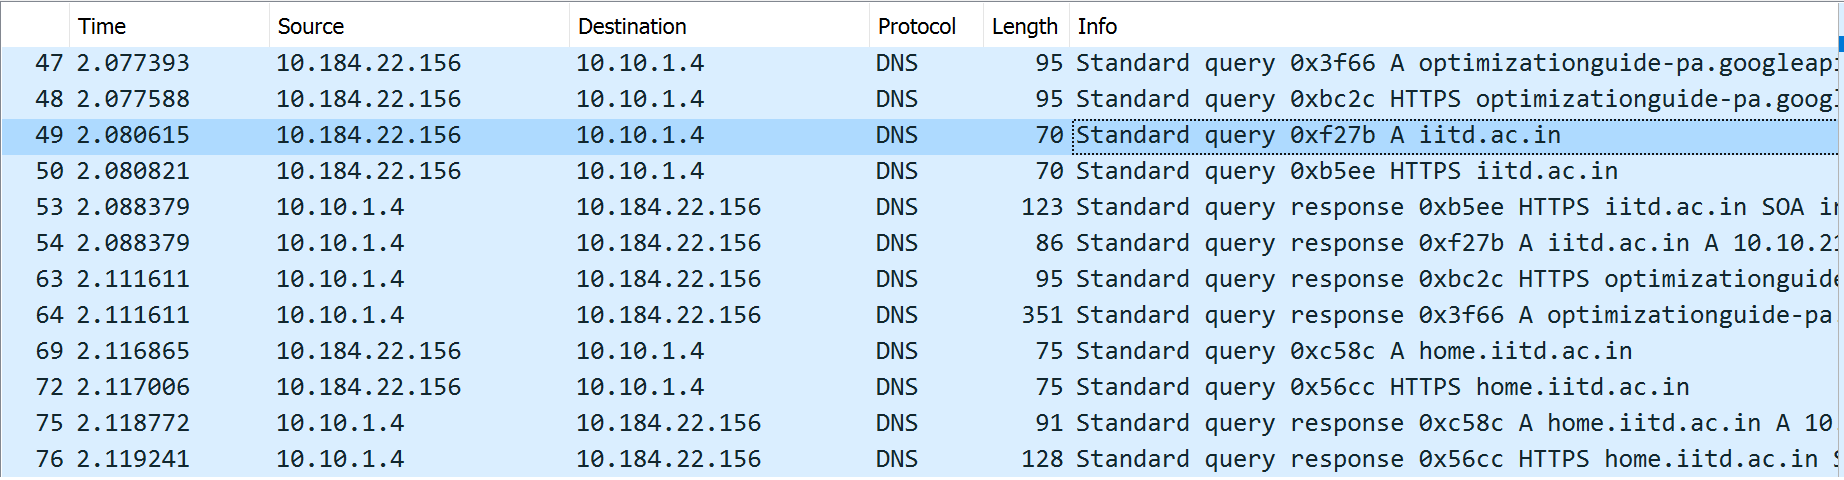
\includegraphics[scale=0.5]{images/IITD dns.png}
        \caption{IITD DNS}
        \label{fig:IITDDNS}
    \end{figure}
    \subsubsection*{Observations}
    As shown in the figure \cref{fig:IITDDNS}, we observe there were DNS queries and responses for {\tt iitd.ac.in}. The request-response began at 2.080615s and ended at 2.088379s lasting for a total of 7.764ms. 

    \item On applying a {\tt http} filter, only one request is observed as shown in \cref{fig:IITDHTTP}
    \begin{figure}[!ht]
        \centering
        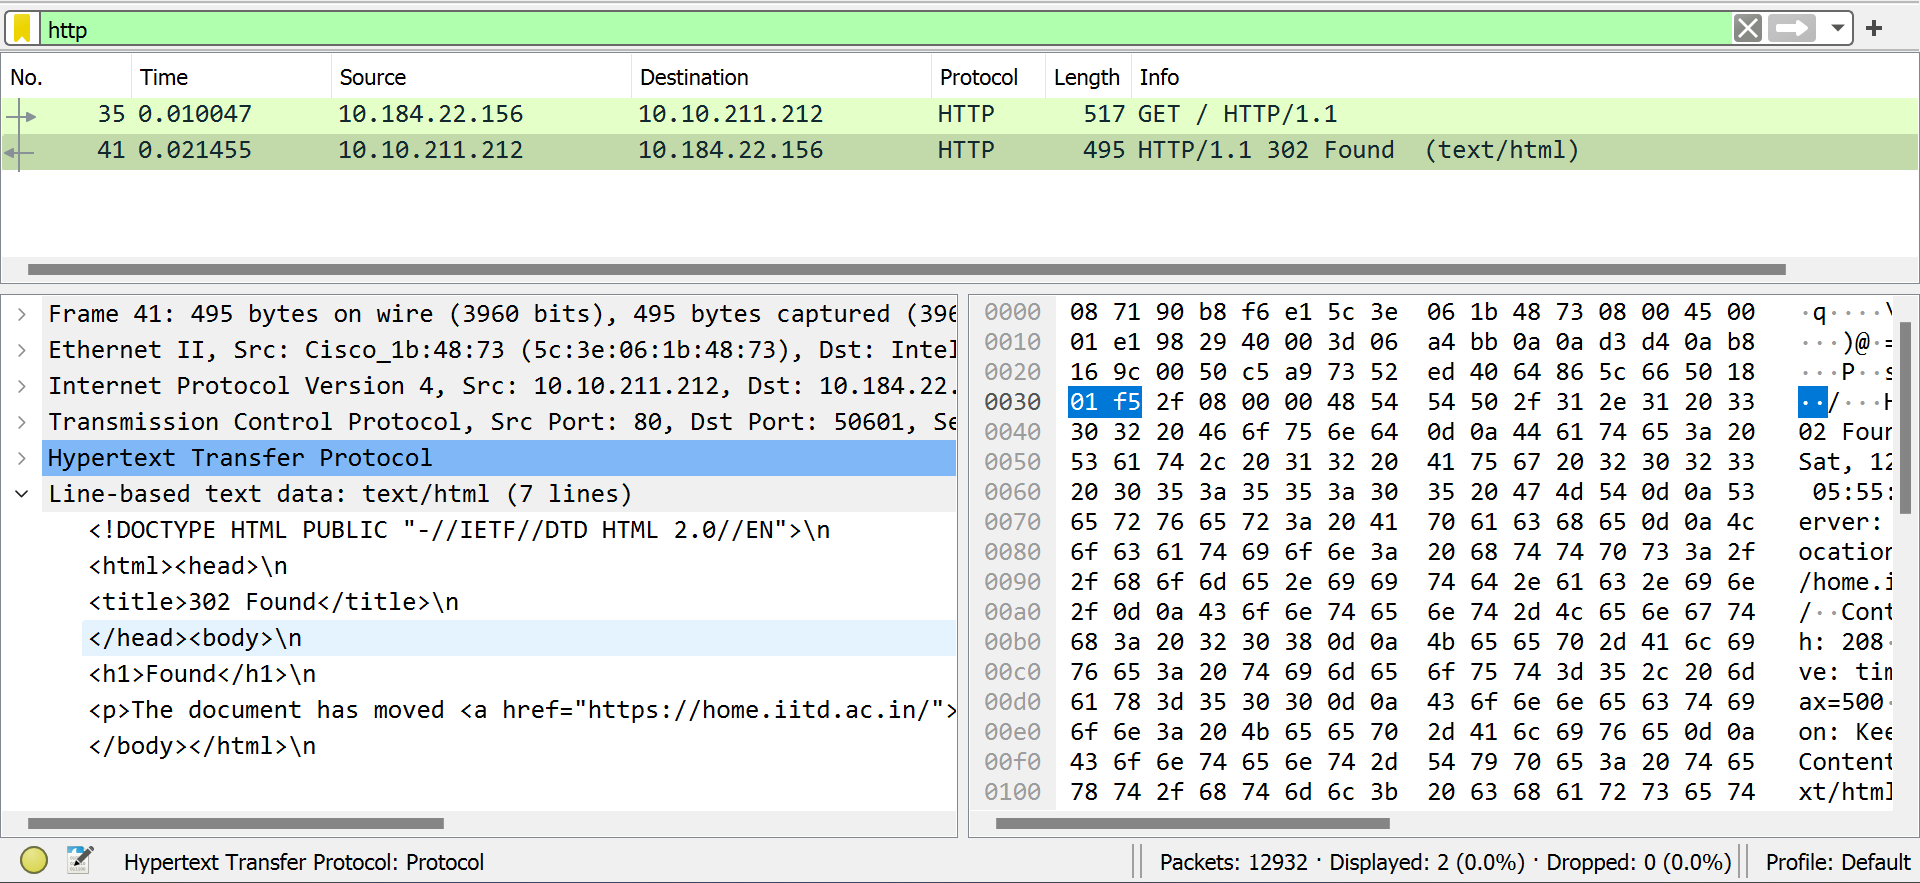
\includegraphics[scale=0.5]{images/IITD http.png}
        \caption{IITD HTTP}
        \label{fig:IITDHTTP}
    \end{figure}
    \subsubsection*{Observations}
    
    \item Next we applied the filter {\tt ((ip.src==10.184.22.156 \&\& ip.dst==10.10.211.212) || (ip.src==10.10.211.212 \&\& ip.dst==10.184.22.156)) \&\& tcp}
\end{enumerate}
\clearpage
\section{Appendix: Preparatory Tasks}
Here, we provide information about the various tools available for network analysis

\subsection{\texttt{ifconfig/ipconfig}}
  This is used to find the following for the network interfaces on the computer:
    \begin{description}
        \item[\textit{IP address}] An IP (Internet Protocol) address is a numerical label assigned to each device connected to a computer network that uses the Internet Protocol for communication. It serves two main purposes: identifying the host or network interface and providing the location of the host in the network. IP addresses can be either IPv4 (32-bit) or IPv6 (128-bit) and are written in a dotted-decimal format (e.g., {\tt172.31.225.222} for IPv4 or {\tt fe80::215:5dff:feeb:19f7} for IPv6).
        \item[\textit{Gateway}] A gateway, often referred to as a default gateway, is a network device (usually a router) that serves as an access point to other networks. It acts as an intermediary between devices within a local network and devices on other networks, including the internet. When a device on a local network wants to communicate with a device on another network, it sends the data to the gateway, which then forwards it to the appropriate destination.
        \item[\textit{Network mask}] A network mask, also known as a subnet mask, is used in conjunction with an IP address to determine the network portion and the host portion of the address. It is a binary pattern of bits that help divide an IP address into a network address and a host address. The network mask is typically represented in decimal format as four octets (e.g., {\tt255.255.255.0} for IPv4). It is used in the process of subnetting to identify which part of the IP address identifies the network and which part identifies the individual host within that network.
        \item[\textit{Hardware address}] A hardware address, also known as a MAC (Media Access Control) address, is a unique identifier assigned to a network interface card (NIC) by its manufacturer. It is a 48-bit address expressed in hexadecimal format and is used to identify a specific device on a local network. Each NIC in the world has its own unique MAC address, allowing devices to communicate with each other at the data link layer of the networking model.
        \item[\textit{DNS server}] A DNS (Domain Name System) server translates human-readable domain names, like www.google.com, into IP addresses that machines can understand. When you enter a URL in a web browser or try to access any internet resource, your device sends a DNS query to a DNS server. The DNS server then looks up the corresponding IP address associated with the domain name and returns it to your device, allowing it to establish a connection to the desired resource.
    \end{description}
    
    Running \texttt{ifconfig} on our system connected to Wifi gives the following output:

        
    \begin{code}
    root@IdeapadAB:~# ifconfig
    eth0: flags=4163<UP,BROADCAST,RUNNING,MULTICAST>  mtu 1500
      inet 172.31.225.222  netmask 255.255.240.0  broadcast 172.31.239.255
      inet6 fe80::215:5dff:feeb:19f7  prefixlen 64  scopeid 0x20<link>
      ether 00:15:5d:eb:19:f7  txqueuelen 1000  (Ethernet)
      RX packets 149  bytes 20663 (20.6 KB)
      RX errors 0  dropped 0  overruns 0  frame 0
      TX packets 13  bytes 1006 (1.0 KB)
      TX errors 0  dropped 0 overruns 0  carrier 0  collisions 0

    lo: flags=73<UP,LOOPBACK,RUNNING>  mtu 65536
      inet 127.0.0.1  netmask 255.0.0.0
      inet6 ::1  prefixlen 128  scopeid 0x10<host>
      loop  txqueuelen 1000  (Local Loopback)
      RX packets 0  bytes 0 (0.0 B)
      RX errors 0  dropped 0  overruns 0  frame 0
      TX packets 0  bytes 0 (0.0 B)
      TX errors 0  dropped 0 overruns 0  carrier 0  collisions 0
    \end{code}

    And on running it on mobile hotspot, we get the following output:
    \begin{code}
    root@IdeapadAB:~# ifconfig
    eth0: flags=4163<UP,BROADCAST,RUNNING,MULTICAST>  mtu 1500
        inet 172.31.225.222  netmask 255.255.240.0  broadcast 172.31.239.255
        inet6 fe80::215:5dff:feeb:19f7  prefixlen 64  scopeid 0x20<link>
        ether 00:15:5d:eb:19:f7  txqueuelen 1000  (Ethernet)
        RX packets 1035  bytes 154375 (154.3 KB)
        RX errors 0  dropped 0  overruns 0  frame 0
        TX packets 103  bytes 8962 (8.9 KB)
        TX errors 0  dropped 0 overruns 0  carrier 0  collisions 0

    lo: flags=73<UP,LOOPBACK,RUNNING>  mtu 65536
        inet 127.0.0.1  netmask 255.0.0.0
        inet6 ::1  prefixlen 128  scopeid 0x10<host>
        loop  txqueuelen 1000  (Local Loopback)
        RX packets 0  bytes 0 (0.0 B)
        RX errors 0  dropped 0  overruns 0  frame 0
        TX packets 0  bytes 0 (0.0 B)
        TX errors 0  dropped 0 overruns 0  carrier 0  collisions 0
    \end{code}

    %%%%%%%%%%%%%%%%%%%%%%% Why is the ip address in both the same? %%%%%%%%%%%%%%%%%%%%%%%

    {\tt eth0} and {\tt lo} are two different network interfaces. {\tt eth0} is associated with the Ethernet connection and {\tt lo} is the loopback(localhost) interface.

    Here is a description of the various fields in the output:
    \begin{description}
        \item[\textit{flags}] A set of flags that indicate the status of the network interface. 
        \item[\textit{mtu}] The Maximum Transmission Unit (MTU) is the size of the largest packet that can be transmitted over the network interface without being fragmented. The MTU is typically measured in bytes and can range from 64 to 65535 bytes.
        \item[\textit{inet}] The IPv4 address assigned to the network interface.
        \item[\textit{netmask}] The subnet mask for the IPv4 address. It helps determine the network and host portions of the IP address.
        \item[\textit{broadcast}] The broadcast address for the network. It is used to send data to all devices on the local network.
        \item[\textit{inet6}] The IPv6 link-local address with a prefix length of 64 bits. IPv6 addresses are written in hexadecimal format and are longer than IPv4 addresses.
        \item[\textit{ether}] The unique hardware address (MAC address) of the network interface card.
        \item[\textit{txqueuelen}] The length of the transmit queue.
        \item[\textit{RX packets}] The number of received packets.
        \item[\textit{TX packets}] The number of transmitted packets.
        \item[\textit{RX errors}] The number of receive errors.
        \item[\textit{TX errors}] The number of transmit errors.
        \item[\textit{dropped}] The number of dropped packets due to errors.
        \item[\textit{overruns}] The number of packets that had data sent beyond their allowed length.
        \item[\textit{frame}] The number of packets with framing errors.
        \item[\textit{collisions}] The number of packet collisions (i.e., when two devices transmit data at the same time).
    \end{description}
    
    The IP address of the smartphone can be found by "Settings$\rightarrow$About phone$\rightarrow$Status$\rightarrow$IP address"

\subsection{\tt ping}
This is used to discover if a particular IP address is online or not. For example, in the following code we are pinging www.google.com with packets of size 10 bytes and varying the TTL. We observe that as the TTL decreases, the packet doesn't reach the destination. This is because the TTL is decremented by 1 at each hop and when it reaches 0, the packet is dropped and an ICMP error message is sent back to the source. The source then knows that the packet didn't reach the destination and hence the destination is not online.
\begin{code}
root@IdeapadAB:~# ping -c 3 -s 50 -t 10 www.google.com
PING www.google.com (142.250.195.4) 50(78) bytes of data.
58 bytes from del12s09-in-f4.1e100.net (142.250.195.4): icmp_seq=1 ttl=55 time=82.3 ms
58 bytes from del12s09-in-f4.1e100.net (142.250.195.4): icmp_seq=2 ttl=55 time=67.1 ms
58 bytes from del12s09-in-f4.1e100.net (142.250.195.4): icmp_seq=3 ttl=55 time=33.1 ms

--- www.google.com ping statistics ---
3 packets transmitted, 3 received, 0% packet loss, time 2004ms
rtt min/avg/max/mdev = 33.130/60.834/82.271/20.545 ms
root@IdeapadAB:~# ping -c 3 -s 50 -t 9 www.google.com
PING www.google.com (142.250.195.4) 50(78) bytes of data.
From 142.251.52.213 (142.251.52.213) icmp_seq=1 Time to live exceeded
From 142.251.52.213 (142.251.52.213) icmp_seq=2 Time to live exceeded
From 142.251.52.213 (142.251.52.213) icmp_seq=3 Time to live exceeded

--- www.google.com ping statistics ---
3 packets transmitted, 0 received, +3 errors, 100% packet loss, time 2299ms
pipe 2
\end{code}



\subsection{\tt traceroute}
This gives you the sequence of routers that a packet traverses to get to a particular destination.
\begin{code}
C:\Users\Anish>tracert iitd.ac.in

Tracing route to iitd.ac.in [103.27.9.24]
over a maximum of 30 hops:

1     3 ms     4 ms     3 ms  192.168.107.98
2    39 ms    29 ms    21 ms  10.50.97.29
3    54 ms    46 ms    23 ms  10.50.97.223
4    58 ms    25 ms    34 ms  10.50.97.77
5   190 ms    30 ms    46 ms  dsl-ncr-dynamic-017.24.23.125.airtelbroadband.in [125.23.24.17]
6    63 ms    37 ms    27 ms  116.119.109.76
7    51 ms    38 ms    26 ms  49.44.187.164
8     *        *        *     Request timed out.
9     *        *        *     Request timed out.
10    38 ms    27 ms    27 ms  136.232.148.178
11     *        *        *     Request timed out.
12     *        *        *     Request timed out.
13     *        *        *     Request timed out.
14    53 ms    36 ms    60 ms  103.27.9.24
15    85 ms    35 ms    36 ms  103.27.9.24
16   148 ms   101 ms    86 ms  103.27.9.24

Trace complete.
\end{code}
\subsection{\tt nslookup}
This command helps you communicate with DNS servers to get the IP address for a particular hostname.

\subsection{\tt nmap}
This is a handy network diagnostics tool that you can use to discover which hosts are online in the network, and even try to infer what operating system the hosts might be running.

\subsection{\tt wireshark}
This is a very useful tool to sniff packets on the wire (or wireless medium). Sniffed data is parsed by wireshark and presented in an easily readable format with details of the protocols being used at different layers.

\end{document}
